%!TEX root = ../bare_adv.tex
%\subsection{Introduction}
Graph-based Modelling~\cite{Jensen:2009:GMB:1590953.1591000} can be used to track the location of objects. 
It uses plans of indoor areas as graphs e.g. as a floor plan of the indoor area. 
This area may be a complex area with several rooms, levels, doors, hallways etc. 
The connectivity and accessibility of the area are represented in as a graph where each room is a vertex and each connection as an edge. 

By representing areas this way, it is possible to track people in the areas from the floor plan, this is done using various low-proximity technologies as Bluetooth, Wi-Fi, RFID etc.

When using a low-proximity technology, the data that is recorded by the sensors, regardless of the technique that is used for this, is saved in a database for later querying and analysis. 
This allows for both Online and Offline tracking.
Online being live querying of the currently available data to see the location of the object, and Offline being a later analysis of the recorded data, if you e.g. want to track the movement pattern of one or more persons. 
To perform online or offline tracking need to three elements: A Deployment Graph, processed sensor data, and the max movement speed of the targeted object.
We now explore these three elements.
This section is largely based on~\cite{Jensen:2009:GMB:1590953.1591000}.

%A Graph-based Model can be applied, as it does not differ between the actual floor plan and the abstract model, hence why using an abstract model provides a equally correct positioning data. 

\subsection{Connectivity, Accessibility, \& Deployment Graphs}
There are three graphs that describes the the topology of a floor plan. 
The first is the \textit{Connectivity Graph} which describes how rooms, hallways, stairs etc. are connected to each other. 
The second is the \textit{Accessibility Graph} which takes the actual accessibility of a cell into account. 
The third is the \textit{Deployment Graph} which contains the rooms and doorways that are equipped with scanners.


\subsubsection{ \quad Connectivity Graph}
Both the Connectivity graph and the Accessibility Graph are constructed based on the actual floor plan. 

\begin{figure}[]%
\centering
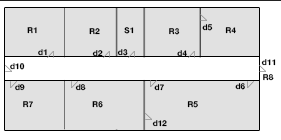
\includegraphics[width=0.8\columnwidth]{images/floorplan.png}%
\caption{Floor plan of a building. Inspired by~\cite{Jensen:2009:GMB:1590953.1591000}}%
\label{fig:floortplan}%
\end{figure}%

Figure \ref{fig:floortplan} shows the floor plan, that is used in our examples.
It contains 7 cells, labelled $R1 - R7$, one staircase labelled $S1$, a hallway and 12 doors labelled $d1-d12$. \\
The area which a cell covers is denoted $A_{cell}$.

In the Connectivity Graph, each separate partitioning of the floor plan (rooms, staircases, hallways etc.) are represented as vertexes, while the connection of these (doors, windows, hatches etc.) are represented as the edges.
E.g. if two rooms are connected by a door, each cell is represented in the base-graph as a vertex, while the door is represented as an undirected edge. 
The Connectivity Graph representing the floor plan from Figure \ref{fig:floortplan} is shown in Figure \ref{fig:connectivitygraph}. 
\begin{figure}[]%
\centering
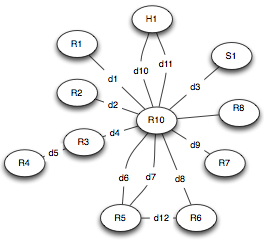
\includegraphics[width=0.8\columnwidth]{images/connectivitygraph.png}%
\caption{Connectivity Graph of the floor plan in Figure \ref{fig:floortplan}.}%
\label{fig:connectivitygraph}%
\end{figure}%
Figure \ref{fig:connectivitygraph} shows how the rooms and hallways in Figure \ref{fig:floortplan} are connected by doors. 
The Connectivity Graph itself is a labelled, undirected multi-graph that is defined by the following triple: \\
\begin{equation}
G_{connection} = (V, E_d, \Sigma_{door})
\end{equation}
In this triple, $V$ is the set of vertexes in the Graph. 
$E_d$ is the set of edges in the Graph, where any edge in $E_d$ is a set consisting of $(\{v_i, v_j\}, k)$ such that $v_i, v_j \in V$ and $k \in \Sigma_{door}$.
Finally, $\Sigma_{door}$ is a set of edge labels that represent the connections. 

%However, it does not make much sense to look at the Connectivity Graph alone when talking about indoor positioning and tracking. 
%To be able to track movement, information about the accessibility of each vertex must also be available. 

\subsubsection{ \quad Accessibility Graph}
There may be situations where a connection does not mean that you have access through that connection.
It can be air-port security or subway ententes that are either entries or exits, which allows one-way movement only.
To take this into account, the Accessibility Graph is used. 
The Accessibility Graph for the floor plan from Figure \ref{fig:floortplan} is shown in Figure \ref{fig:accesibbilitygraph}.
\begin{figure}[]%
\centering
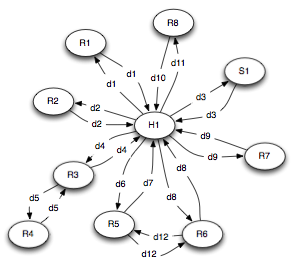
\includegraphics[width=0.8\columnwidth]{images/accessibilitygraph.png}%
\caption{Accesibility graph of the floor plan in Figure \ref{fig:floortplan}.} % and the connectivity graph in Figure \ref{fig:floortplan}.}%
\label{fig:accesibbilitygraph}%
\end{figure}%
Figure \ref{fig:accesibbilitygraph} shows the Accessibility Graph.
It can be seen that door $d10$ only allows entrance from outside and into the hall, while door $d11$ only allows exit from the hall.
The Accessibility Graph is a labelled, directed graph and constructed to represent available movement patterns in the area. \\
An Accessibility Graph $G_{access}$ is given by the triple: 
\begin{equation}
G_{access} = (V, E, \Sigma_{door}, l_e)
\end{equation} 
where $V$ is the set of vertexes, $E$ is the set of directed edges, having $E = \{\langle v_i, v_j \rangle | v_i, v_j \in V,  v_i \not= v_j\}$ and finally $l_e$ is a function that maps edges to subsets of the doors, having $l_e : E \rightarrow 2^{\Sigma_{door}}$. \\

%These graphs provide an abstract representation of the floor plan, which -- combined with the previously mentioned logging -- will allow for indoor movement tracking and indoor positioning. 

\subsubsection{ \quad Deployment Graph}
While the Accessibility Graph is based on the Connectivity Graph, the Deployment Graph is based on the Accessibility Graph. 
The Deployment Graph is an Accessibility graph where edges is doors with sensors e.g. if two rooms do not have a sensor at the passage door then the two rooms are view as the same room.
%When it is known in what direction people can travel, it is possible to make deployment plan for the sensors to read movement patterns. 
%This scenario is based on RFID technology that uses proximity analysis for determining when a tag is approaching a reader. 
%All RFID readers must have disjoint activations ranges, meaning that a tag cannot be read by more than one reader at the time. \\
The actual deployment varies from case to case. 
There are two kind of readers. 
Partitioning readers and Presence readers. \\

The partitioning readers partition the indoor space into different cells. 
An object cannot move from one cell to another without being read by a sensor. 
When deploying partitioning readers, one can choose between placing one or two readers in every door opening. 
By placing one reader only, it is not possible to track which way the object is moving - only that is has been recorded passing the reader in question. 
%In order to find out in which way the object was moving, the history of other reads of the same object has to be taken into account. 
By placing two readers in every door opening, it is possible to detect in which direction the object is moving (e.g. if it is moving in or out of the cell). \\

Presence readers are readers that do not contribute to the partitioning of the indoor space. 
They simply observe which objects are present within its range. 
%These recordings will also have an entry- and an exit time of when the any given object enters or exists the readers range. \\

A deployment graph should be complete, meaning that it should capture all present cells and connections between them, and it should have as few vertices and edges as possible. \\
An RFID deployment graph is represented as a directed, labelled graph:
\begin{equation}
G_{RFID} = (C, E_r, \Sigma_{reader}, l_e)
\end{equation} 
where $C$ is the set of vertixes, $E_r$ is the set of edges (an edge is an ordered pair $\langle c_i, c_j \rangle$ of distinct vertexes from $C$) and $l_e : E_r \rightarrow 2^{\Sigma_{reader}} \cup 2^{\Sigma_{reader} X \Sigma_{reader}}$ maps an edge to a partitioning reader or a partitioning reader pair. \\

The Deployment Graph is a map of how readers are located in an indoor area. 

%\IEEEPARstart{T}{his} demo file is intended to serve as a ``starter file''
%for IEEE Computer Society journal papers produced under \LaTeX\ using
%IEEEtran.cls version 1.7 and later.
% You must have at least 2 lines in the paragraph with the drop letter
% (should never be an issue)
%I wish you the best of success.
%\hfill mds
%\hfill January 11, 2007
